% Chapter Template

\chapter{Generalizing the Numerical Solution Using Fourier Solution}

\label{Chapter8} % Change X to a consecutive number; for referencing this chapter elsewhere, use \ref{ChapterX}

\lhead{Chapter 8. \emph{Generalizing the Fourier Numerical Solution}}

\section{Why?}
The problem with trying to plot out the fourier solution upto a certain number of frequencies is that, the fourier coefficients need to calculated separately for each type of problem. This is cumbersome and thus it is of value to search for a solution which id general and doesn't require us to hand-calculate each time.
\section{Solution - Fast Fourier Transform}
To solve this equation using the Fast Fourier Transform (FFT), we take the Fourier transform of both sides. The Fourier transform of a time-domain function $f(t)$ is defined as:
\begin{align}
    F(\omega) = \int_{-\infty}^{\infty} f(t) e^{-j\omega t} dt
\end{align}
Applying this to the given differential equation, we use the property that the Fourier transform of a derivative is given by:
\begin{align}
    \mathcal{F} \left( \frac{df}{dt} \right) = j\omega F(\omega)
\end{align}
Taking the Fourier transform of both sides:
\begin{align}
    L (j\omega I(\omega)) + R I(\omega) = V(\omega)
\end{align}
Rearranging for $I(\omega)$:
\begin{align}
    I(\omega) = \frac{V(\omega)}{R + j\omega L}
\end{align}
To obtain $i(t)$ in the time domain, we take the inverse Fourier transform:
\begin{align}
    i(t) = \mathcal{F}^{-1} \left( I(\omega) \right) = \mathcal{F}^{-1} \left( \frac{V(\omega)}{R + j\omega L} \right)
\end{align}
The inverse Fourier transform is computed numerically using the Inverse Fast Fourier Transform (IFFT) in practical implementations. This step allows us to reconstruct the time-domain current response from the frequency-domain solution.
To solve this equation using the Fast Fourier Transform (FFT), we take the Fourier transform of both sides. The Fourier transform of a time-domain function $f(t)$ is defined as:
\begin{align}
    F(\omega) = \int_{-\infty}^{\infty} f(t) e^{-j\omega t} dt
\end{align}
Applying this to the given differential equation, we use the property that the Fourier transform of a derivative is given by:
\begin{align}
    \mathcal{F} \left( \frac{df}{dt} \right) = j\omega F(\omega)
\end{align}
Taking the Fourier transform of both sides:
\begin{align}
    L (j\omega I(\omega)) + R I(\omega) = V(\omega)
\end{align}
Rearranging for $I(\omega)$:
\begin{align}
    I(\omega) = \frac{V(\omega)}{R + j\omega L}
\end{align}
To obtain $i(t)$ in the time domain, we take the inverse Fourier transform:
\begin{align}
    i(t) = \mathcal{F}^{-1} \left( I(\omega) \right) = \mathcal{F}^{-1} \left( \frac{V(\omega)}{R + j\omega L} \right)
\end{align}
The inverse Fourier transform is computed numerically using the Inverse Fast Fourier Transform (IFFT) in practical implementations. This step allows us to reconstruct the time-domain current response from the frequency-domain solution.
\section{Effects of sampling}
We use several different ranges of sampling frequency to see which is "good" enough.
     \begin{center}
          Below Nyquist Rate $(f_s < 2 f_{\max})$: 
     \end{center}
    \captionsetup{type=figure}
    \centering
    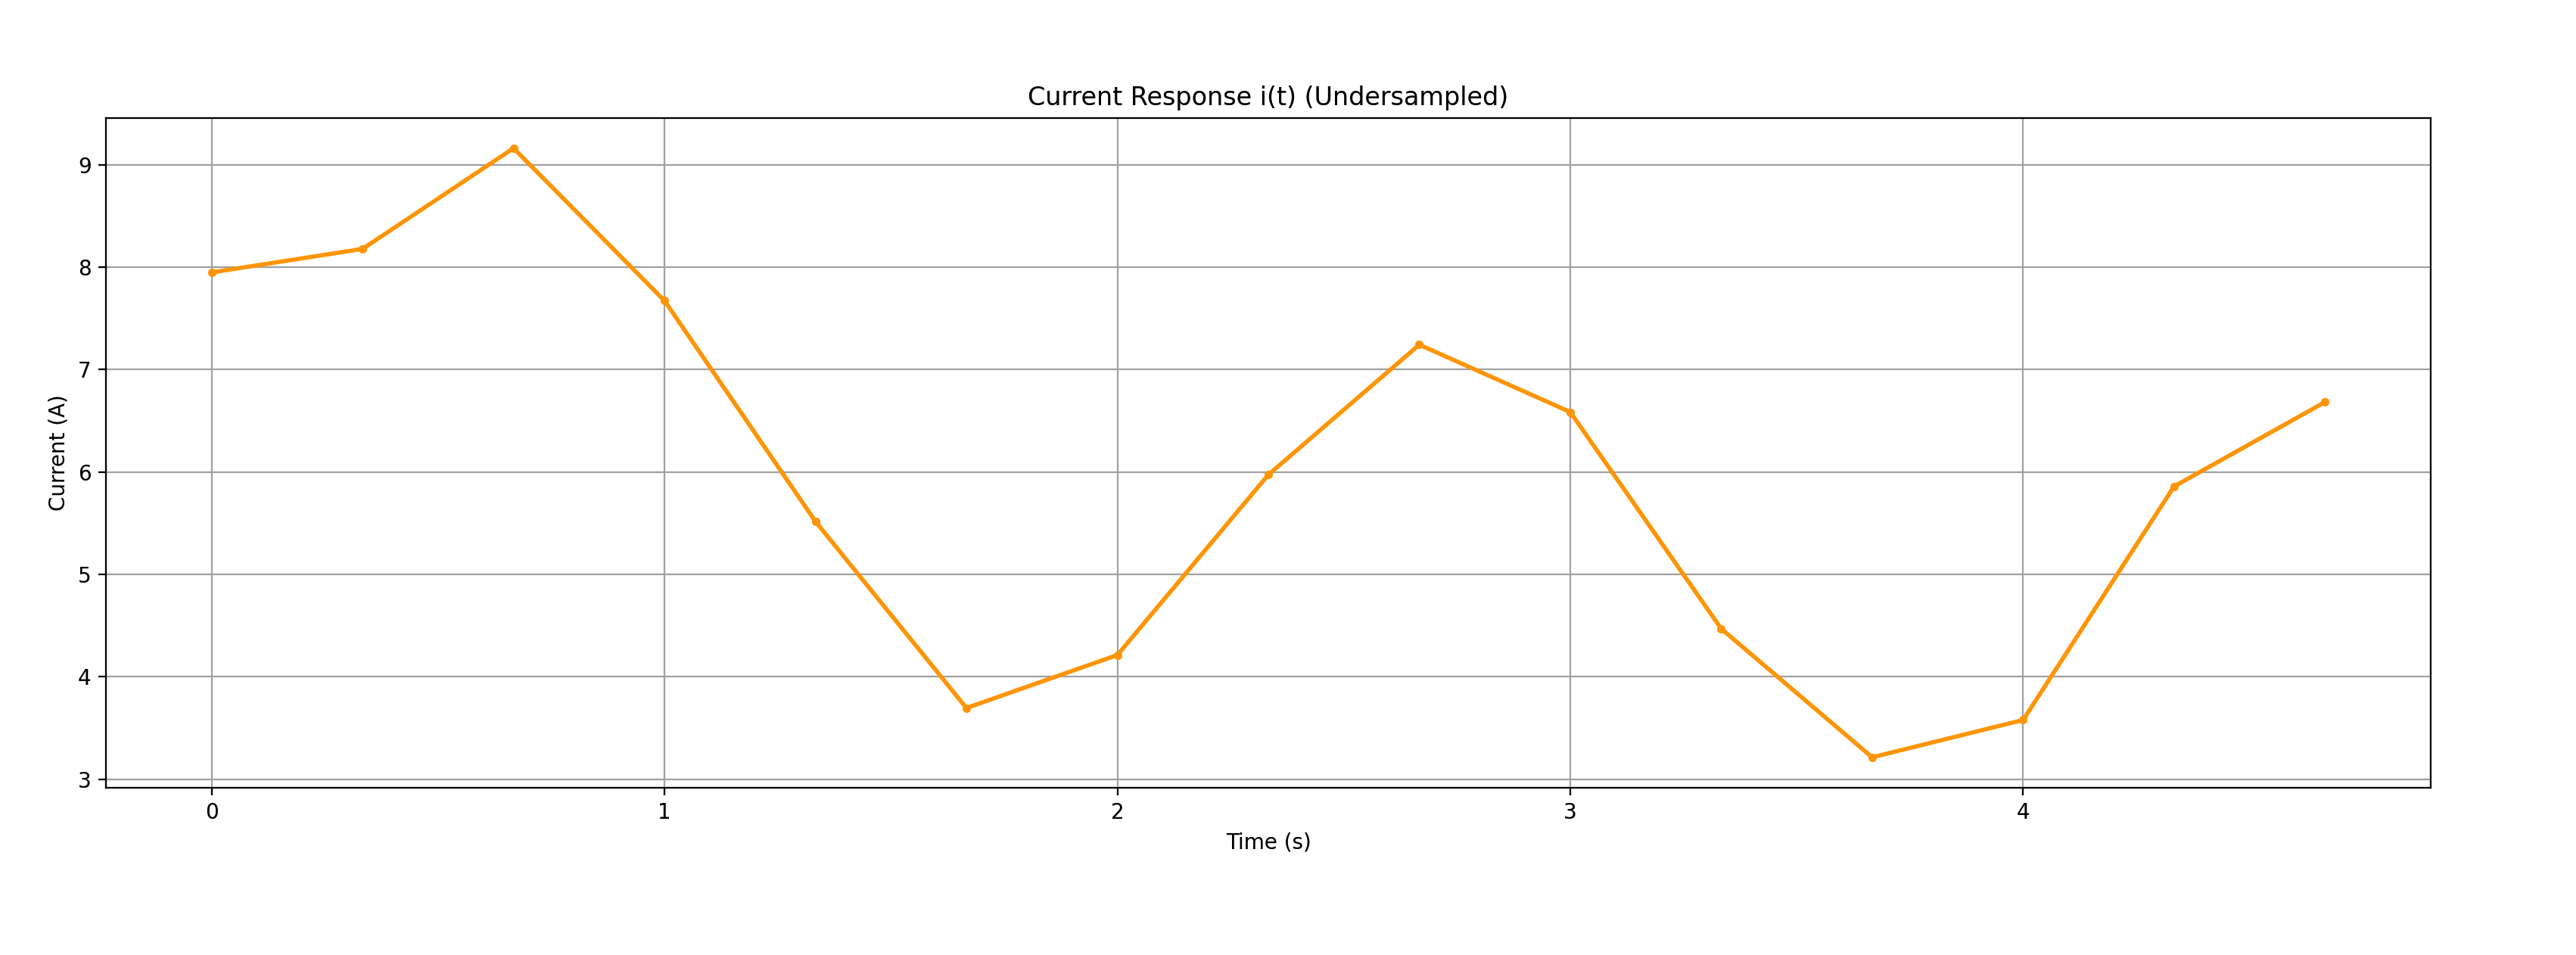
\includegraphics[width=0.6\textwidth]{figs/0_75f_ny.png}
    \caption{The current response for  $f_s < f_{ny}$   i.e, $(0.75*f_{ny})$}
    \label{fig:example}
      \begin{itemize}
          \item The square wave appears distorted, with missing transitions or incorrect duty cycle representation.
          \item The FFT spectrum shows incorrect frequency content.
      \end{itemize}
    \begin{center}  
      Slightly Above Nyquist Rate: 
    \end{center}
      
      \captionsetup{type=figure}
    \centering
    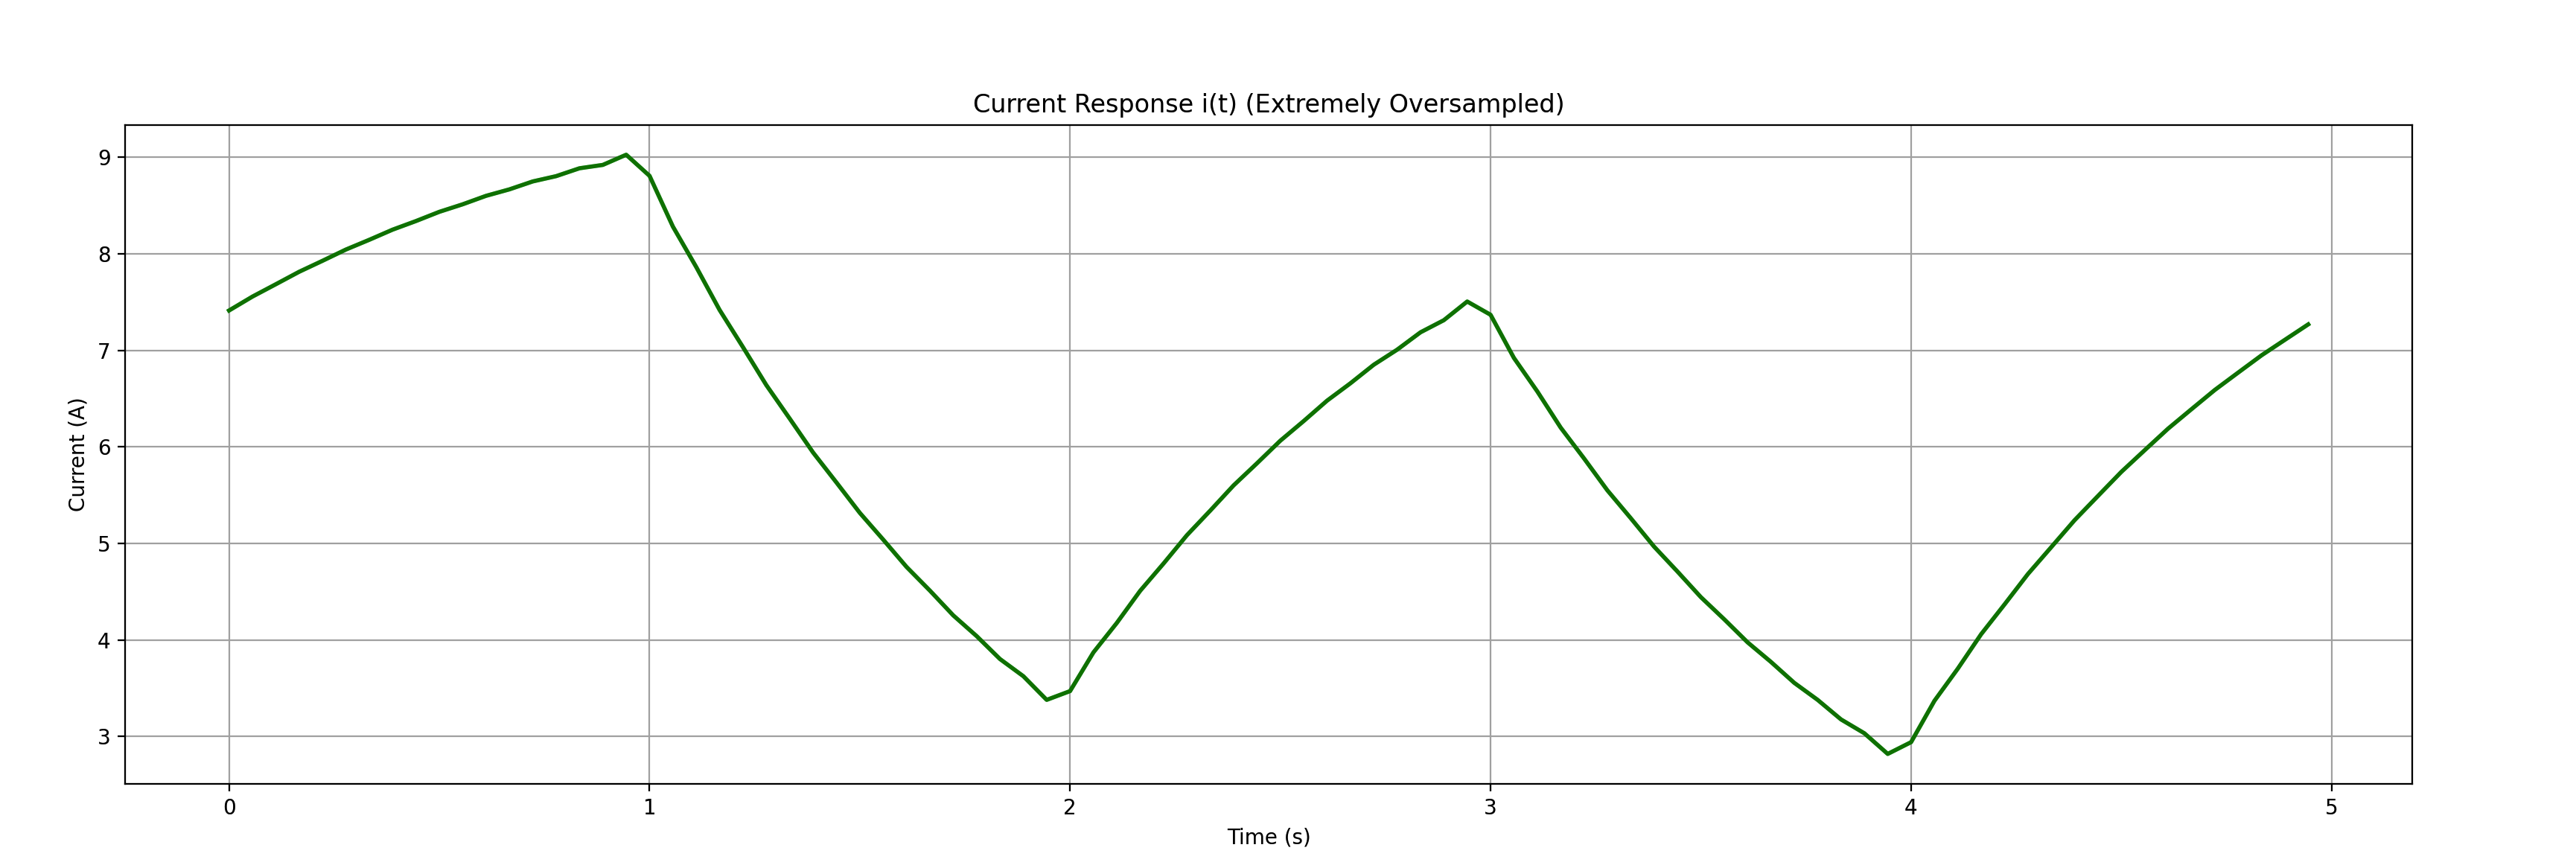
\includegraphics[width=0.6\textwidth]{figs/4_f_ny.png}
    \caption{The current response for  $f_s > f_{ny}$   i.e, $(4f_{ny})$}
    \label{fig:example}
    \begin{itemize}
        \item The waveform is well-preserved, and the current response $i(t)$ matches expected results.
        \item Harmonic content is properly captured.
    \end{itemize}
    \begin{center} 
     Very High Sampling Rate $(f_s \gg 2 f_{\max}):$
    \end{center}
     \captionsetup{type=figure}
    \centering
    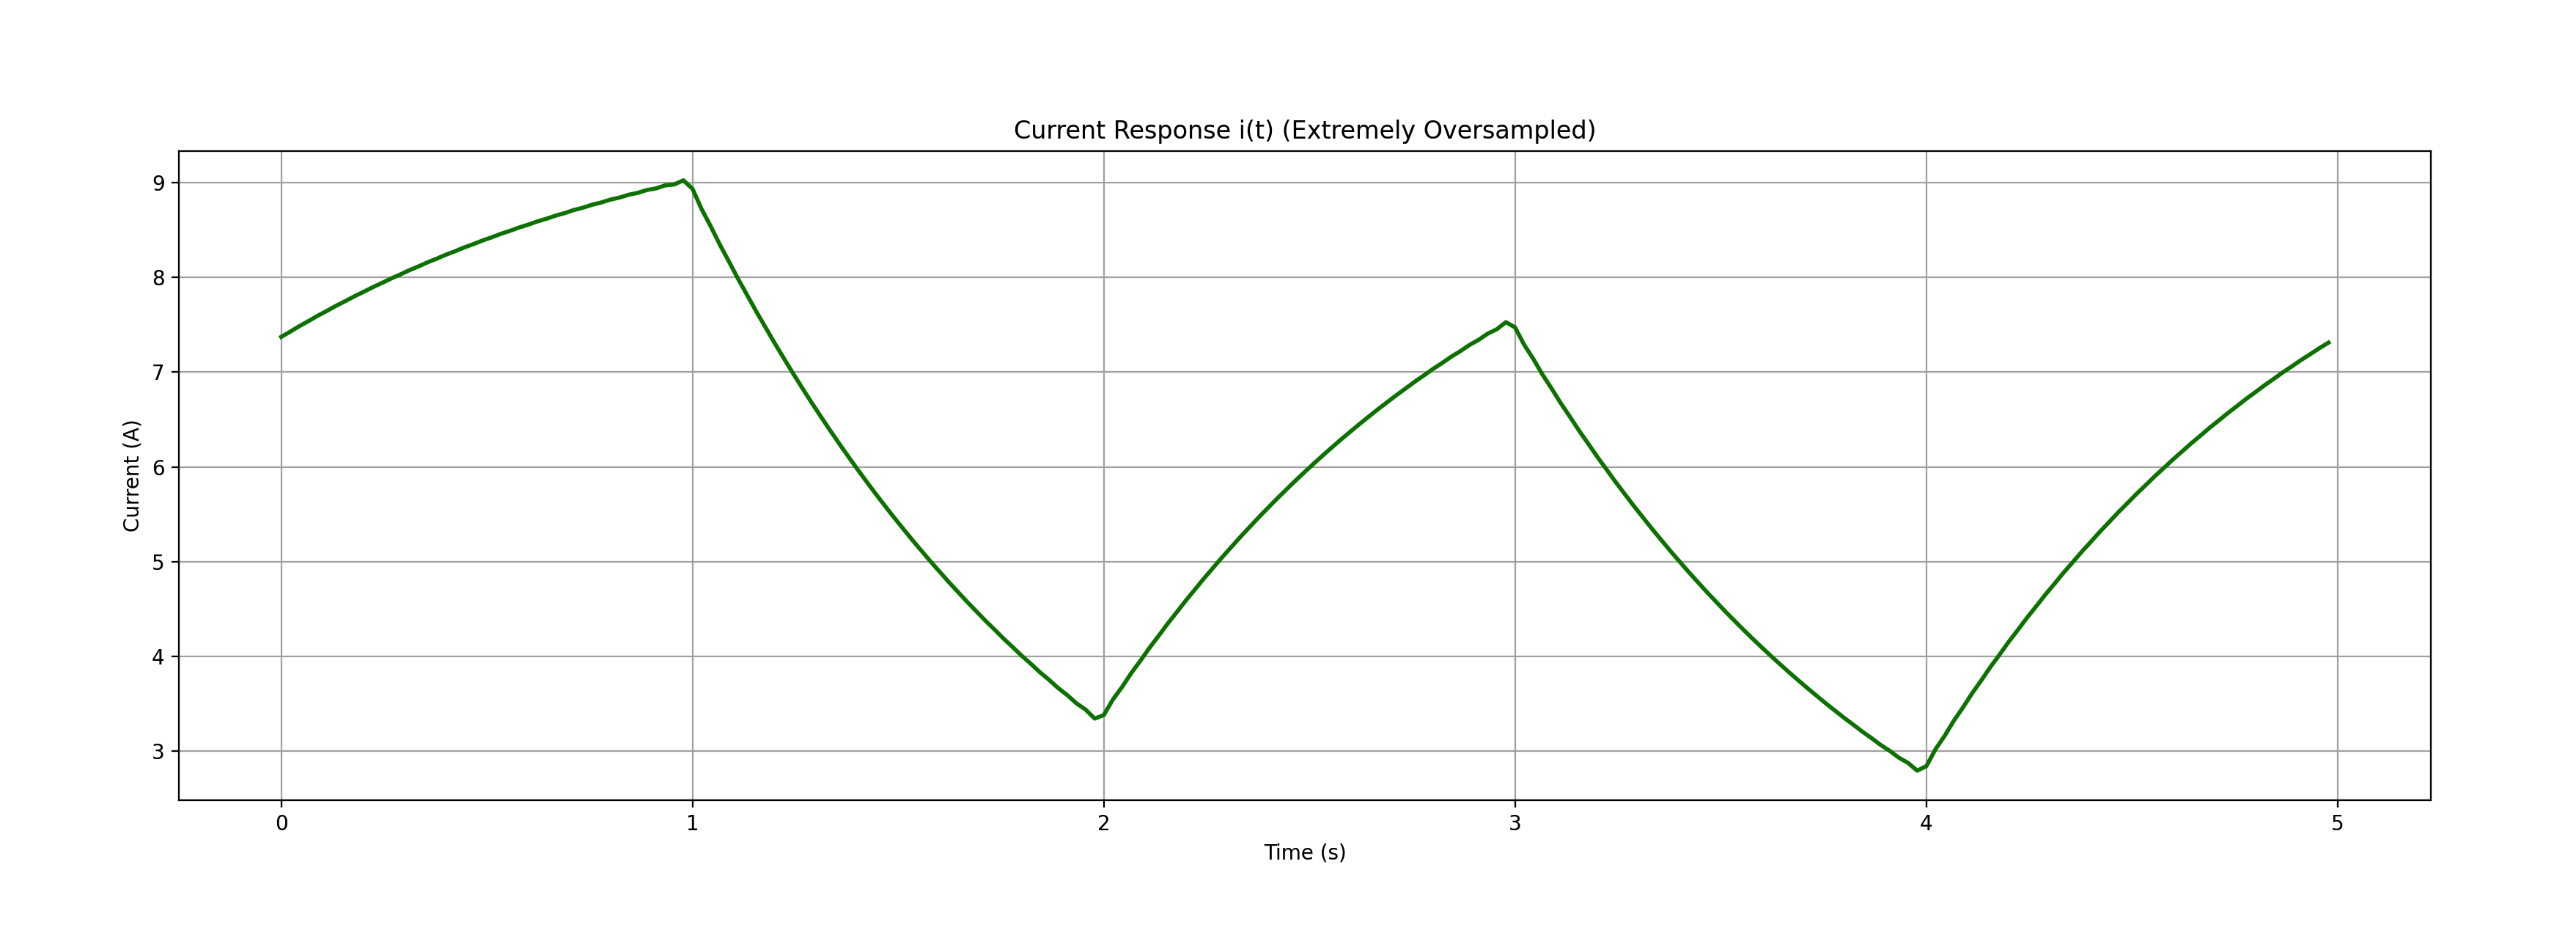
\includegraphics[width=0.6\textwidth]{figs/10_f_ny.png}
    \caption{The current response for  $f_s \gg f_{ny}$   i.e, $(10 f_{ny})$}
    \label{fig:example}
    \begin{itemize}
        \item 	No significant change in the output waveform is observed.
        \item Computation time increases, but results remain nearly the same.
    \end{itemize}
    So it is evident that something about the frequency corresponding to twice the frequency of input wave is special. This special nature is captured by the \textbf{sampling theorem}.

\section{Key Findings: }
\begin{enumerate}
    \item FFT-Based Solution for RL Circuits:
    \begin{itemize}
        \item The FFT method provides an efficient way to analyze linear circuit responses in the frequency domain.
        \item By applying the inverse FFT, we accurately retrieve the time-domain current response.
    \end{itemize}
    \item Nyquist Sampling and Computational Efficiency:
    \begin{itemize}
        \item Sampling at or above the Nyquist rate preserves essential frequency components while minimizing data redundancy.
        \item Increasing the sampling rate beyond a certain threshold does not significantly alter the output current waveform, confirming the sufficiency of Nyquist's criterion.
    \end{itemize}
    \item Effect of Circuit Parameters:
    \begin{itemize}
        \item The RL circuit acts as a low-pass filter, smoothing the square wave input by attenuating higher harmonics.
        \item he response shape is influenced by the resistance R, inductance L, and the duty cycle of the input square wave.
    \end{itemize}
    \item Practical Implications:
    \begin{itemize}
        \item Understanding sampling limitations is crucial for real-world signal processing and embedded systems applications.
        \item The interactive implementation enables real-time visualization of how different parameters affect the circuit's behavior.
    \end{itemize}
\end{enumerate}